\documentclass[11pt,aspectratio=1610]{beamer}

\usepackage[spanish,es-nodecimaldot]{babel}
\usepackage[utf8]{inputenc}
\usepackage[T1]{fontenc}
\usepackage{amsmath,amssymb,bm}
\usepackage{tikz}
\usepackage{graphicx}
\usepackage{booktabs}
\usepackage{array}
\usepackage{xcolor}
\usepackage{ragged2e}
\usepackage{hyperref}

\usetheme{Madrid}
\setbeamertemplate{navigation symbols}{}

\definecolor{UAOrange}{HTML}{D37229}
\definecolor{UABlue}{HTML}{2B437B}
\definecolor{UABlueLight}{HTML}{6F86B3}
\definecolor{White}{HTML}{FFFFFF}
\definecolor{LightGray}{HTML}{F4F5F7}
\definecolor{DarkGray}{HTML}{333333}

\setbeamercolor{structure}{fg=UABlue}
\setbeamercolor{normal text}{fg=DarkGray,bg=White}
\setbeamercolor{background canvas}{bg=White}
\setbeamercolor{palette primary}{fg=White,bg=UABlue}
\setbeamercolor{palette secondary}{fg=White,bg=UABlue}
\setbeamercolor{palette tertiary}{fg=White,bg=UAOrange}
\setbeamercolor{palette quaternary}{fg=White,bg=UABlue}
\setbeamercolor{frametitle}{fg=White,bg=UABlue}
\setbeamerfont{frametitle}{size=\large,series=\bfseries}
\setbeamercolor{block title}{fg=White,bg=UABlue}
\setbeamercolor{block body}{fg=DarkGray,bg=LightGray}
\setbeamercolor{block title alerted}{fg=White,bg=UAOrange}
\setbeamercolor{block body alerted}{fg=DarkGray,bg=UAOrange!10}
\setbeamercolor{block title example}{fg=White,bg=UABlueLight}
\setbeamercolor{block body example}{fg=DarkGray,bg=UABlueLight!10}
\setbeamercolor{math text}{fg=UABlue}

\setbeamertemplate{footline}{%
  \leavevmode
  \hbox{%
    \begin{beamercolorbox}[wd=.30\paperwidth,ht=3ex,dp=1.2ex,leftskip=0.5cm]{author in head/foot}
      \usebeamerfont{author in head/foot}\insertshortauthor
    \end{beamercolorbox}%
    \begin{beamercolorbox}[wd=.50\paperwidth,ht=3ex,dp=1.2ex,center]{title in head/foot}
      \usebeamerfont{title in head/foot}\insertshorttitle
    \end{beamercolorbox}%
    \begin{beamercolorbox}[wd=.20\paperwidth,ht=3ex,dp=1.2ex,center]{date in head/foot}
      \color{White}\insertframenumber/\inserttotalframenumber
    \end{beamercolorbox}%
  }
}
\setbeamercolor{author in head/foot}{fg=White,bg=UABlue}
\setbeamercolor{title in head/foot}{fg=White,bg=UABlue}
\setbeamercolor{date in head/foot}{fg=White,bg=UAOrange}

\setbeamertemplate{headline}{%
  \ifnum\insertframenumber>1
    \begin{tikzpicture}[remember picture,overlay]
      \node[anchor=north east,xshift=-0.25cm,yshift=-0.12cm] at (current page.north east) {%
        \IfFileExists{UA.png}{
\includegraphics[height=0.55cm]{UA.png}}{}
      };
    \end{tikzpicture}
  \fi
}

\setbeamertemplate{frametitle}{%
  \nointerlineskip
  \begin{beamercolorbox}[wd=\paperwidth,ht=1.05cm,dp=0.25cm,leftskip=0.45cm]{frametitle}
    \usebeamerfont{frametitle}\insertframetitle
  \end{beamercolorbox}
}

\setbeamerfont{title}{size=\LARGE,series=\bfseries}
\setbeamerfont{subtitle}{size=\large}
\setbeamerfont{author}{size=\normalsize}
\setbeamerfont{institute}{size=\small}

\title[Radiación sincrotrón]{El gran sincrotrón del Caribe: un paso que debemos dar}
\subtitle{Radiación de sincrotrón: la luz que desentraña los secretos íntimos de la materia}
\author[Frailen MOS - Alejandro D]{Frailen Ojeda \\ Alejandro De León}
\institute[Universidad del Atlántico]{Universidad del Atlántico\\Facultad de Ciencias Básicas\\Programa de Física}
\date{Septiembre de 2026}

\begin{document}

{\setbeamertemplate{footline}{}\setbeamertemplate{headline}{}
\begin{frame}
  \begin{tikzpicture}[remember picture,overlay]
    \fill[UABlue] (current page.south west) rectangle (current page.north east);
    \fill[White] ([xshift=11.0cm]current page.north west) -- (current page.north east) -- (current page.south east) -- ([xshift=9.2cm]current page.south west) -- cycle;
    \fill[UAOrange] ([xshift=10.65cm]current page.north west) -- ([xshift=11.15cm]current page.north west) -- ([xshift=9.35cm]current page.south west) -- ([xshift=8.85cm]current page.south west) -- cycle;
    \fill[White] (current page.south west) -- ([xshift=7.0cm]current page.south west) -- ([xshift=8.0cm,yshift=0.75cm]current page.south west) -- ([yshift=0.75cm]current page.south east) -- (current page.south east) -- cycle;
    \fill[UAOrange] (current page.south west) rectangle ([yshift=0.16cm]current page.south east);
    \fill[UAOrange] ([xshift=0.8cm,yshift=-1.65cm]current page.north west) rectangle ([xshift=0.87cm,yshift=-4.75cm]current page.north west);
  \end{tikzpicture}

  \begin{tikzpicture}[remember picture,overlay]
    \node[anchor=west,text=White,align=left,text width=8.8cm,font=\bfseries] at ([xshift=1.05cm,yshift=-2.35cm]current page.north west) {\fontsize{27}{31}\selectfont El gran sincrotrón\\ del Caribe};
    \node[anchor=west,text=White,align=left,text width=8cm,font=\fontsize{16}{20}\selectfont] at ([xshift=1.05cm,yshift=-4.05cm]current page.north west) {un paso que debemos dar};
    \node[anchor=west,text=White!85,align=left,text width=7.5cm,font=\small] at ([xshift=1.05cm,yshift=-4.85cm]current page.north west) {La luz que desentraña los secretos íntimos de la materia};
    \IfFileExists{UA.png}{\node[anchor=center] at ([xshift=13.15cm,yshift=-4.7cm]current page.north west) {
\includegraphics[width=3.2cm]{UA.png}};}{ }
    \node[anchor=center,text=UABlue,align=center,font=\small] at ([xshift=12.8cm,yshift=-7.15cm]current page.north west) {{\bfseries UNIVERSIDAD DEL ATLÁNTICO}\\[0.10cm] Facultad de Ciencias Básicas\\ Programa de Física};
    \node[anchor=south west,text=White,align=left] at ([xshift=1cm,yshift=1cm]current page.south west) {{\normalsize\bfseries Frailen Ojeda \quad | \quad Alejandro De León}\\[0.3em]{\footnotesize Septiembre de 2026}};
  \end{tikzpicture}
\end{frame}}

\begin{frame}{Contenido}
  \tableofcontents
\end{frame}

\section{Introducción}
\begin{frame}{Introducción}
  \begin{columns}[T]
    \column{0.5\textwidth}
      \centering
      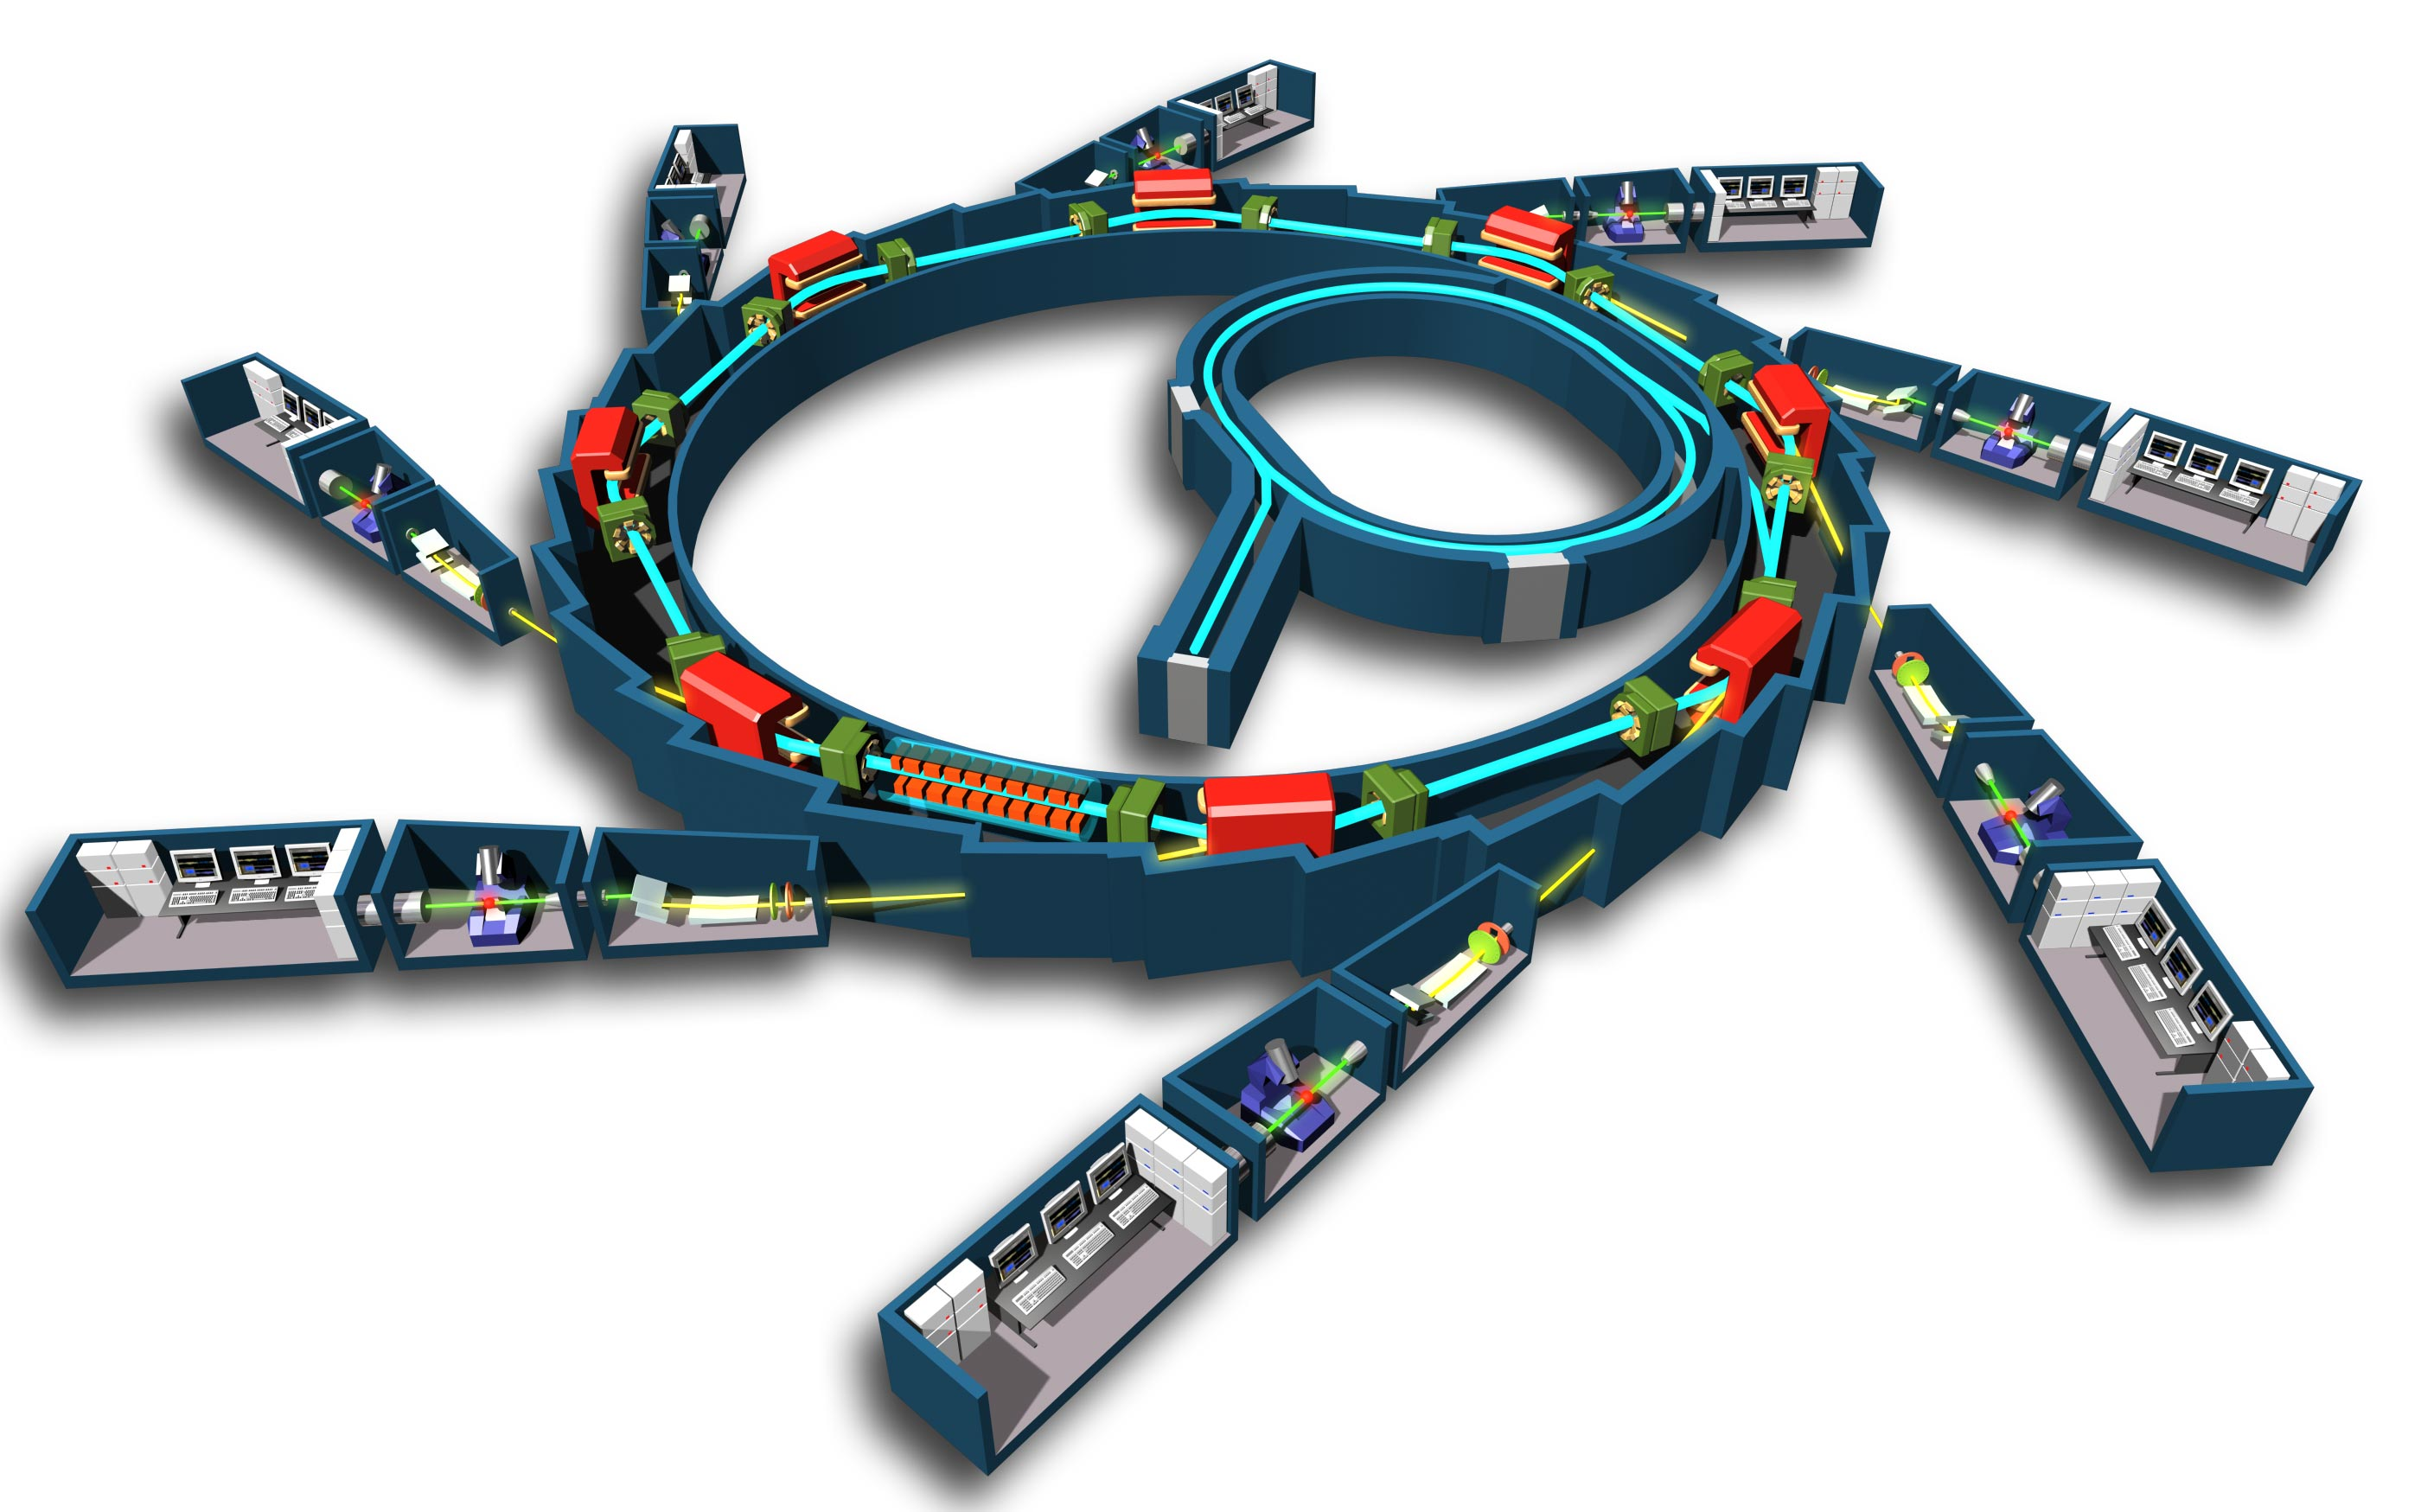
\includegraphics[width=0.8\linewidth]{sincrtrón.jpg}
      \small $^1$Diagrama de un sincrotrón
      \vspace{0.4cm}
      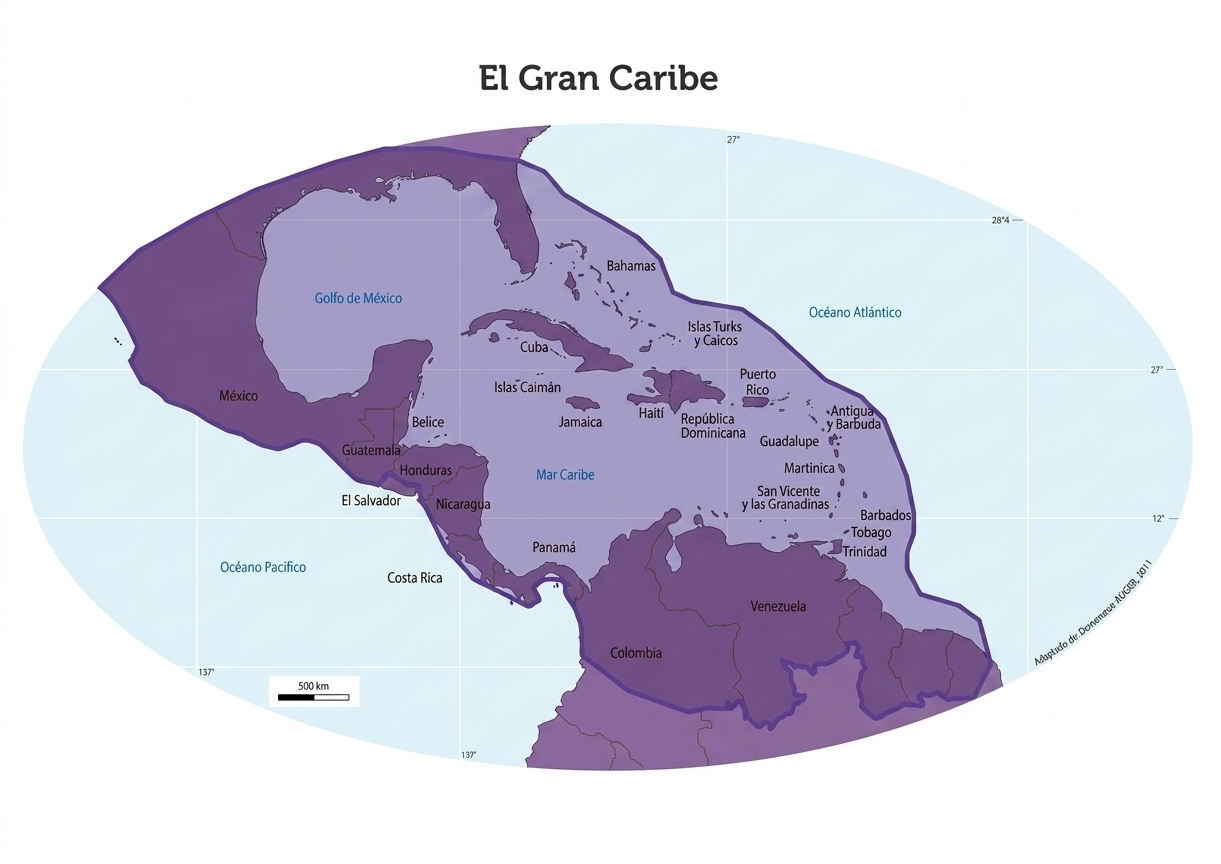
\includegraphics[width=0.6\linewidth]{elgrancaribe.jpeg}

    \column{0.5\textwidth}
      \centering
      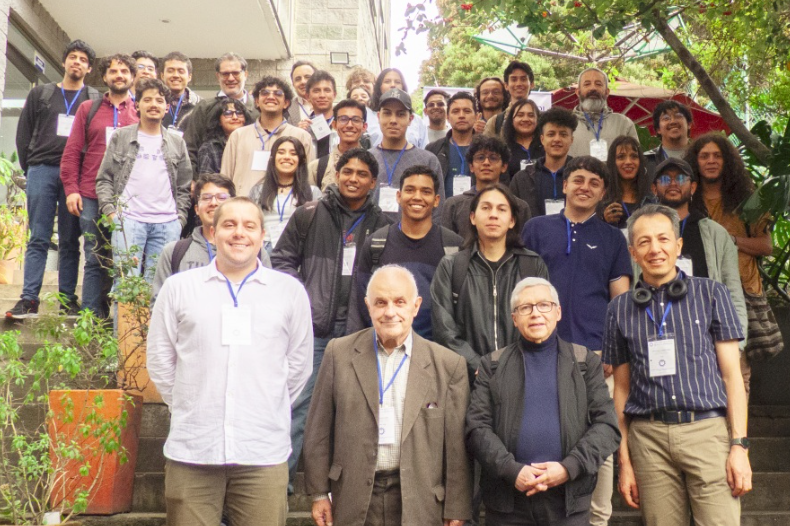
\includegraphics[width=0.9\linewidth]{foto.png}
      \vspace{5mm}
      
\includegraphics[width=0.9\linewidth]{AbdusSalam.png}
  \end{columns}
  \footnotetext[1]{Tomada de \textit{Synchrotron SOLEIL -- EPSIM 3D/J.-F. Santarelli} (2005).}
\end{frame}

\section{¿Cómo funciona un sincrotrón?}
\begin{frame}{¿Cómo se aceleran las partículas?}
  \framesubtitle{Cavidad resonante}
  \begin{columns}
    \column{0.48\textwidth}
      \centering
      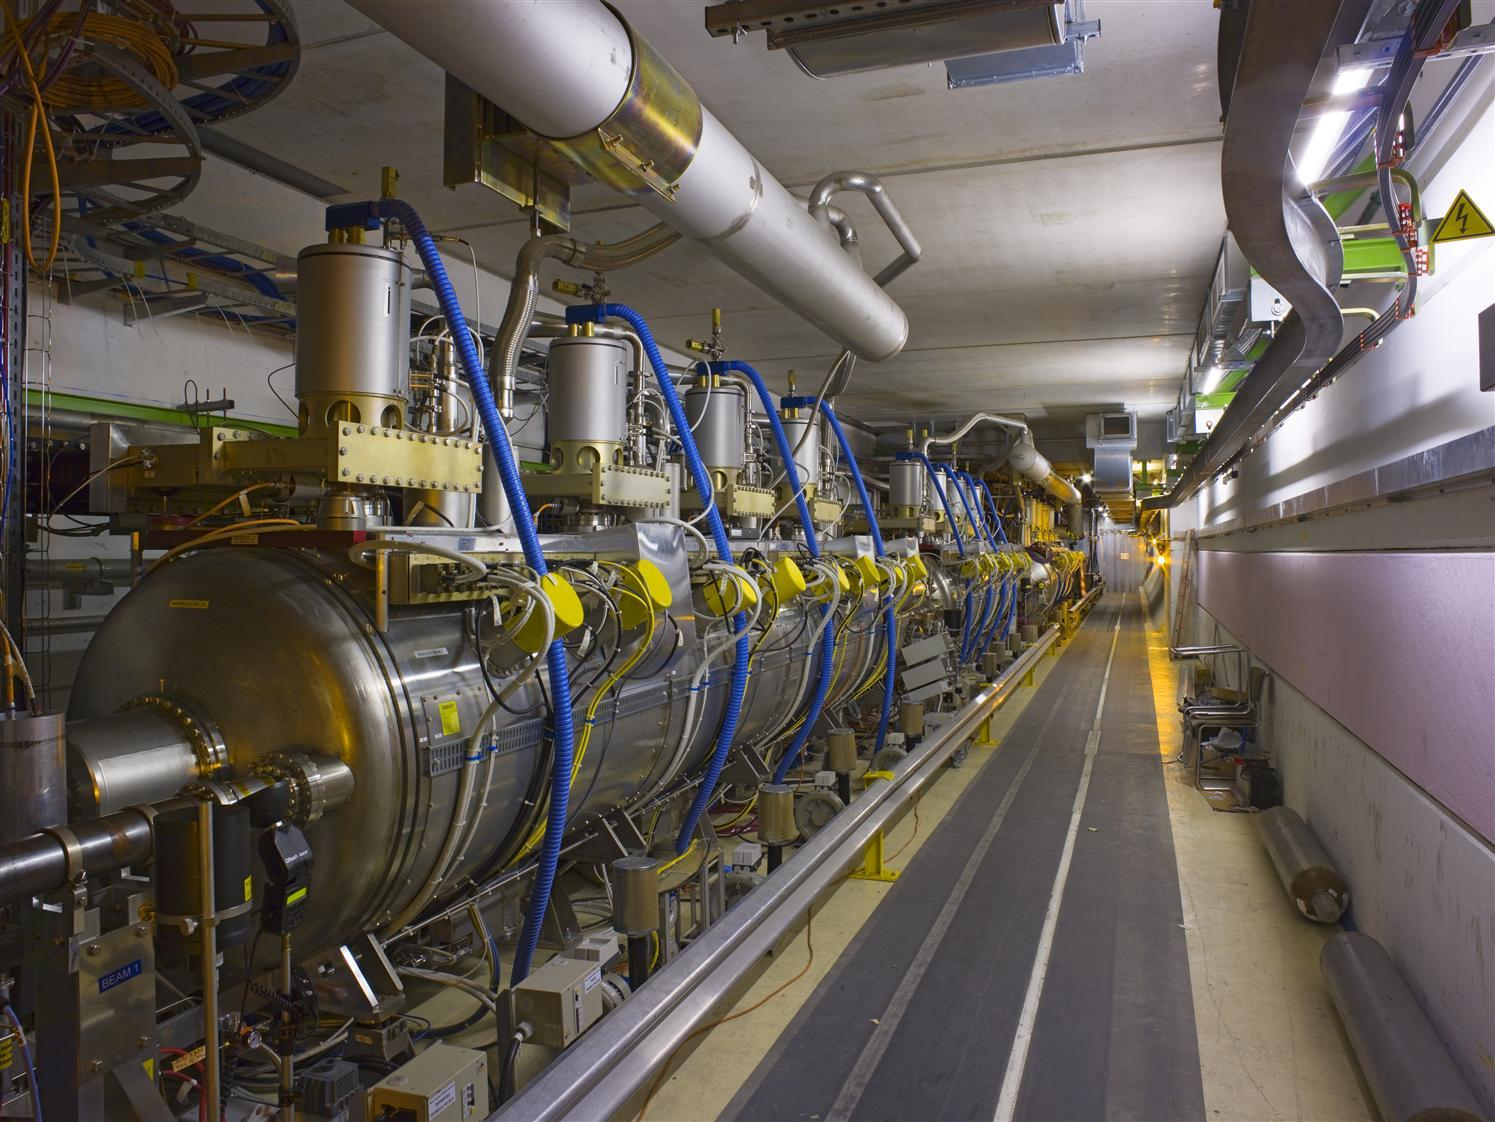
\includegraphics[width=0.85\linewidth]{LHC.png}
      \parbox{0.85\linewidth}{\centering\scriptsize $^2$ Cavidad de radiofrecuencia superconductora del LHC.}

    \column{0.52\textwidth}
      \centering
      \[\boxed{\vec{E}(t)=\vec{E}_0\cos(\omega_{\mathrm{RF}}t+\phi)}\]
      \begin{block}{RF}
        En la cavidad, el campo eléctrico longitudinal es el que realiza trabajo sobre la partícula.
      \end{block}
      \[\boxed{\Delta E = qV_0\cos(\omega_{\mathrm{RF}}t+\phi)}\]
  \end{columns}
  \footnotetext[2]{CERN, \textit{Radiofrequency cavities}.}
\end{frame}

\begin{frame}{Geometría de la cavidad de radiofrecuencia superconductora}
  \begin{columns}
    \column{0.4\textwidth}
      \centering
      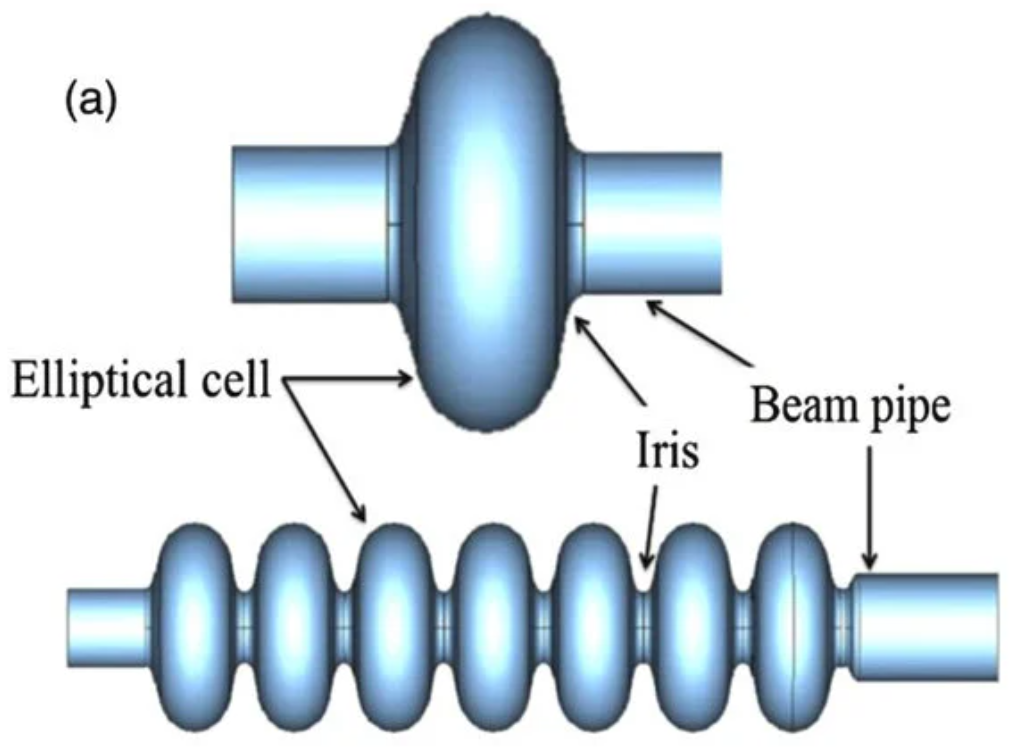
\includegraphics[width=\linewidth]{RF-diagrama.png}
      \par\vspace{0.1cm}
      \small $^5$Diagrama de la cavidad RF

    \column{0.6\textwidth}
      \centering
      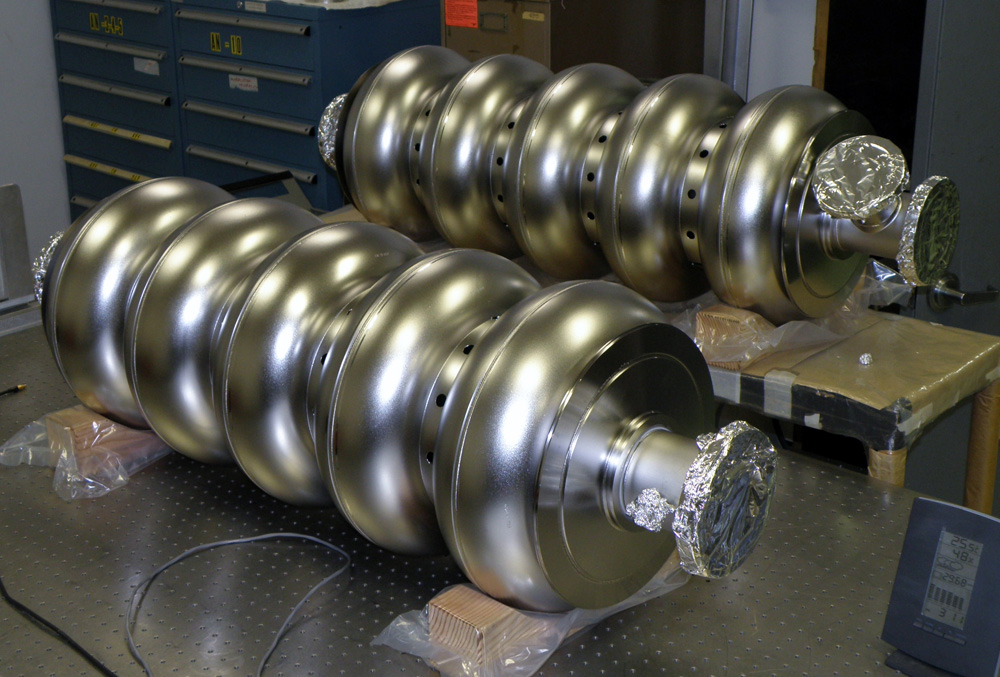
\includegraphics[width=\linewidth]{RF-Fermilab.jpg}
      \par\vspace{0.1cm}
      \small $^4$Cavidades superconductoras de radiofrecuencia de cinco celdas
  \end{columns}
  \footnotetext[4]{Tomado de \href{https://pip2.fnal.gov/how-it-works/superconducting-radio-frequency-technology/}{\textit{Fermilab PIP-II}}.}
  \footnotetext[5]{\href{https://doi.org/10.1103/PhysRevAccelBeams.26.092001}{Shemelin \& Yakovlev. \textit{Phys. Rev. Accel. Beams} \textbf{26}, 092001 (2023).}}
\end{frame}

\begin{frame}{Trayectoria de las partículas cargadas}
  \begin{block}{Pregunta}
    ¿Cómo desviamos la trayectoria de una partícula cargada?
  \end{block}
  \begin{columns}
    \column{0.5\textwidth}
      \centering
      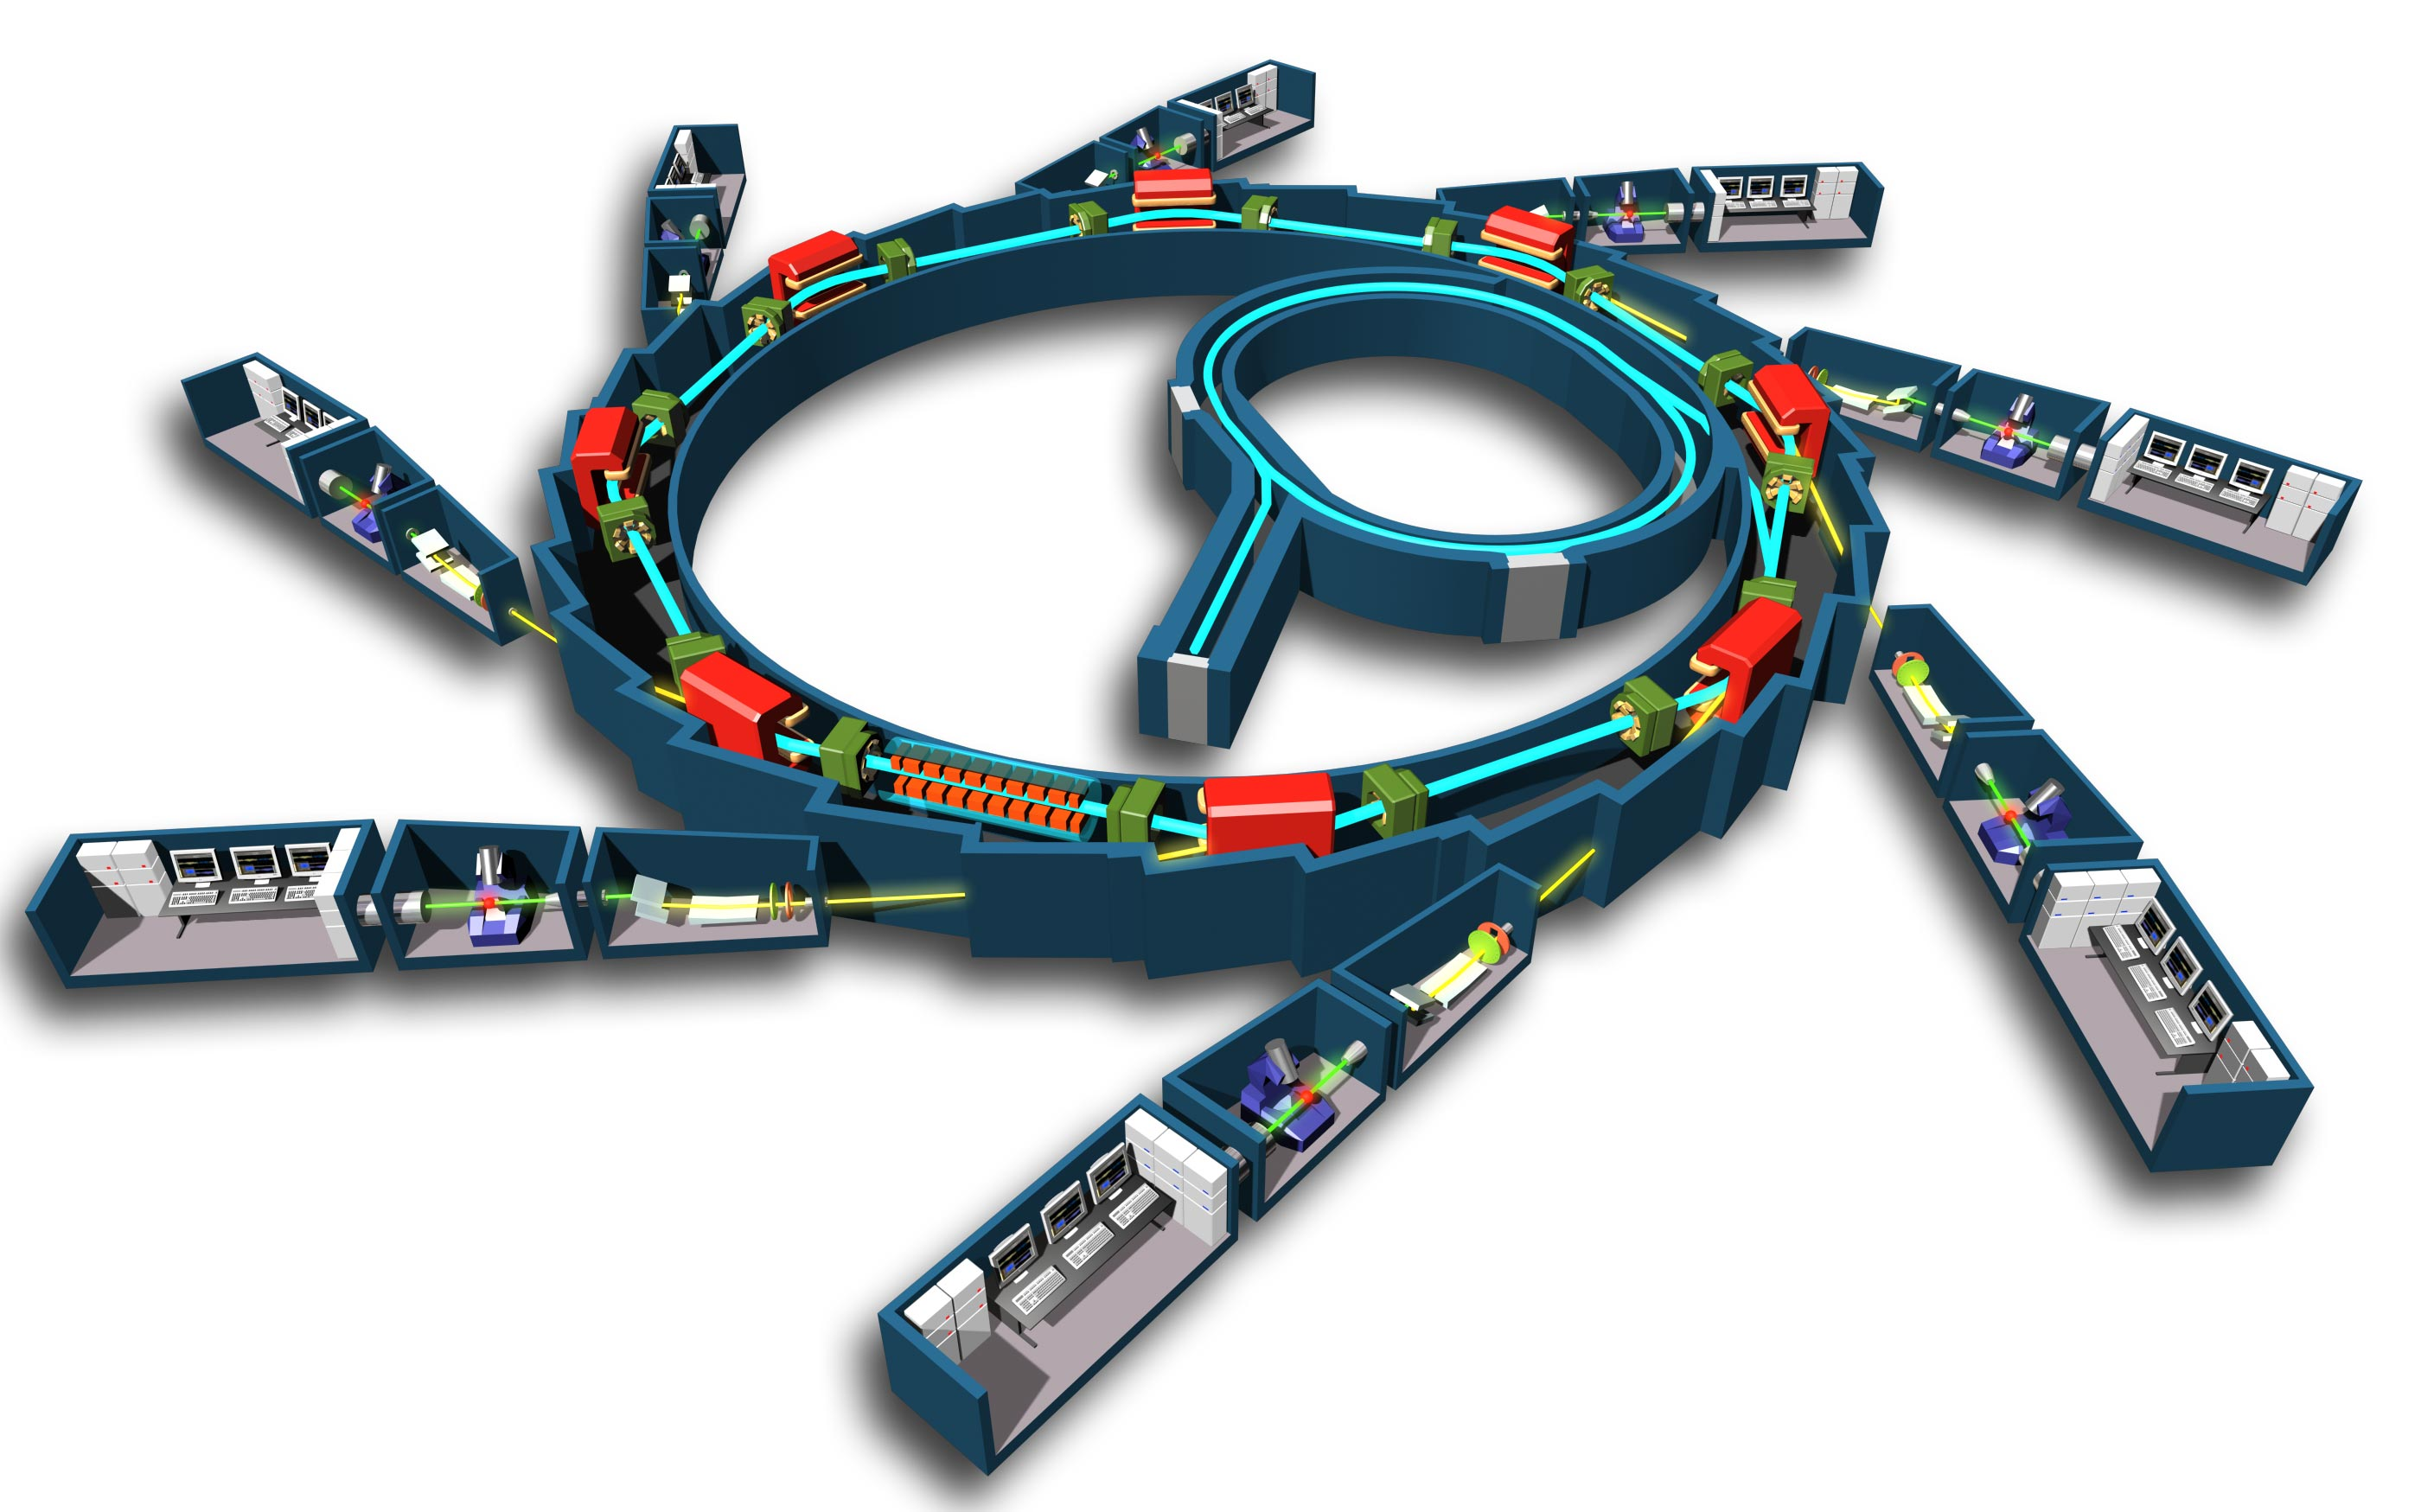
\includegraphics[width=0.9\linewidth]{sincrtrón.jpg}
      \small $^1$Diagrama de un sincrotrón

    \column{0.5\textwidth}
      \centering
      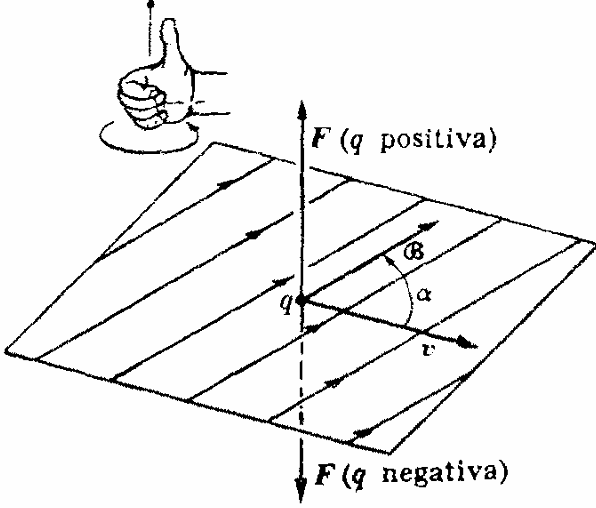
\includegraphics[width=0.7\linewidth]{carga en campo.png}
      \parbox{0.9\linewidth}{\justifying\scriptsize $^6$Relación vectorial entre la fuerza magnética, el campo magnético y la velocidad de la carga.}
  \end{columns}
  \footnotetext[1]{Tomada de \textit{Synchrotron SOLEIL -- EPSIM 3D/J.-F. Santarelli} (2005).}
  \footnotetext[6]{Tomado de \textit{Alonso \& Finn, Física Vol2}.}
\end{frame}

\begin{frame}{Imanes dentro del sincrotrón}
  \begin{columns}[T]
    \column{0.3333\textwidth}
      \centering
      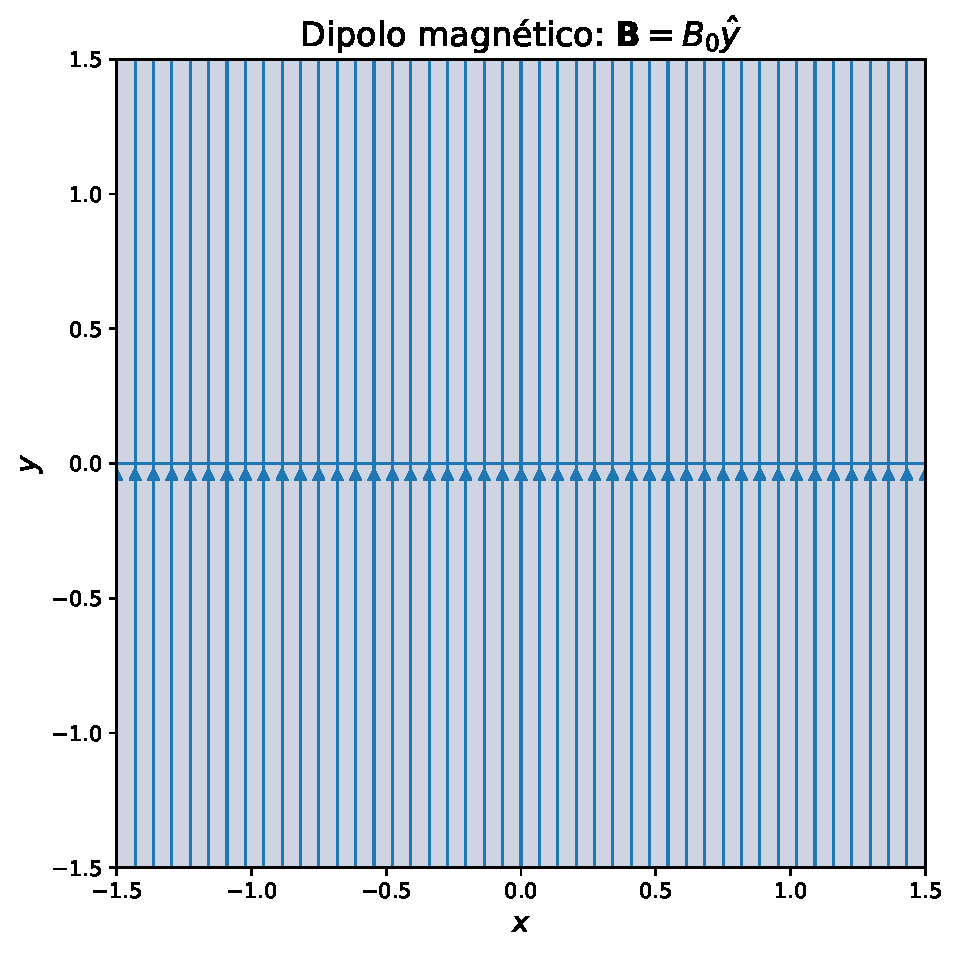
\includegraphics[width=0.85\linewidth]{dipolo_magnetico.pdf}
      \vspace{0.2cm}
      \textbf{Dipolo}
      \vspace{0.1cm}\small Curvatura del haz

    \column{0.3333\textwidth}
      \centering
      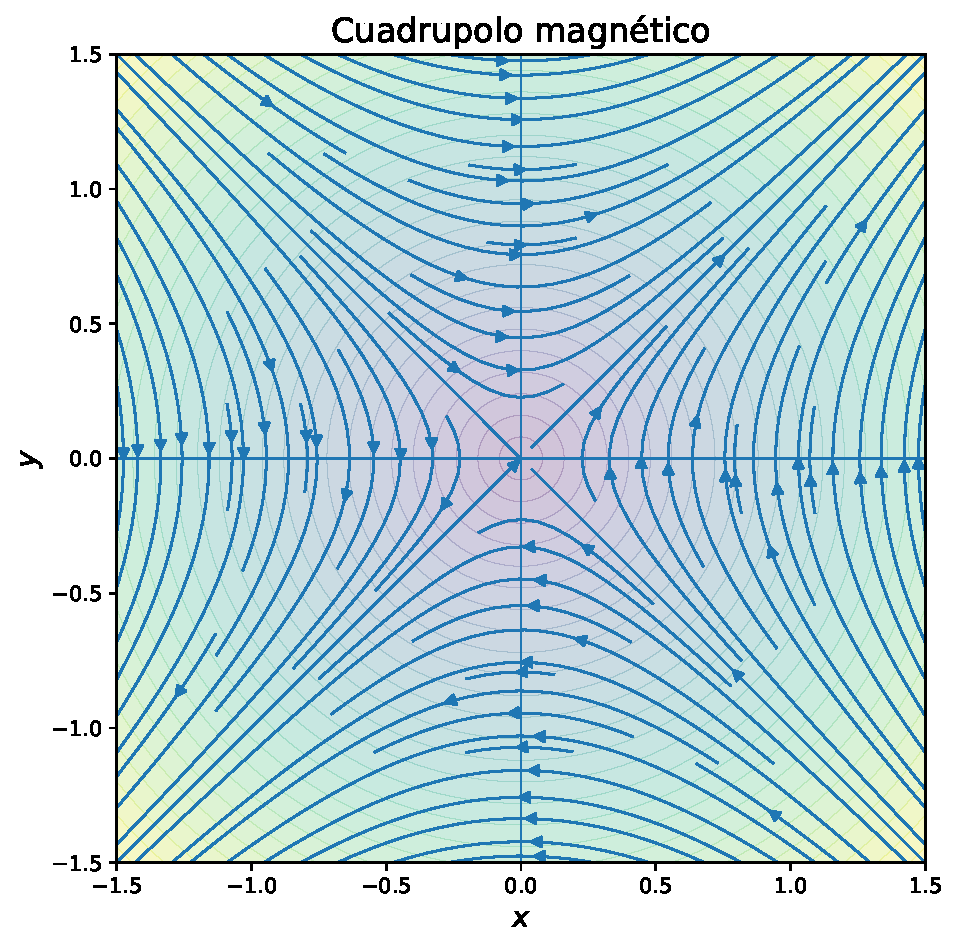
\includegraphics[width=0.85\linewidth]{cuadrupolo_magnetico.pdf}
      \vspace{0.2cm}
      \textbf{Cuadrupolo}
      \vspace{0.1cm}\small Enfoque del haz

    \column{0.3333\textwidth}
      \centering
      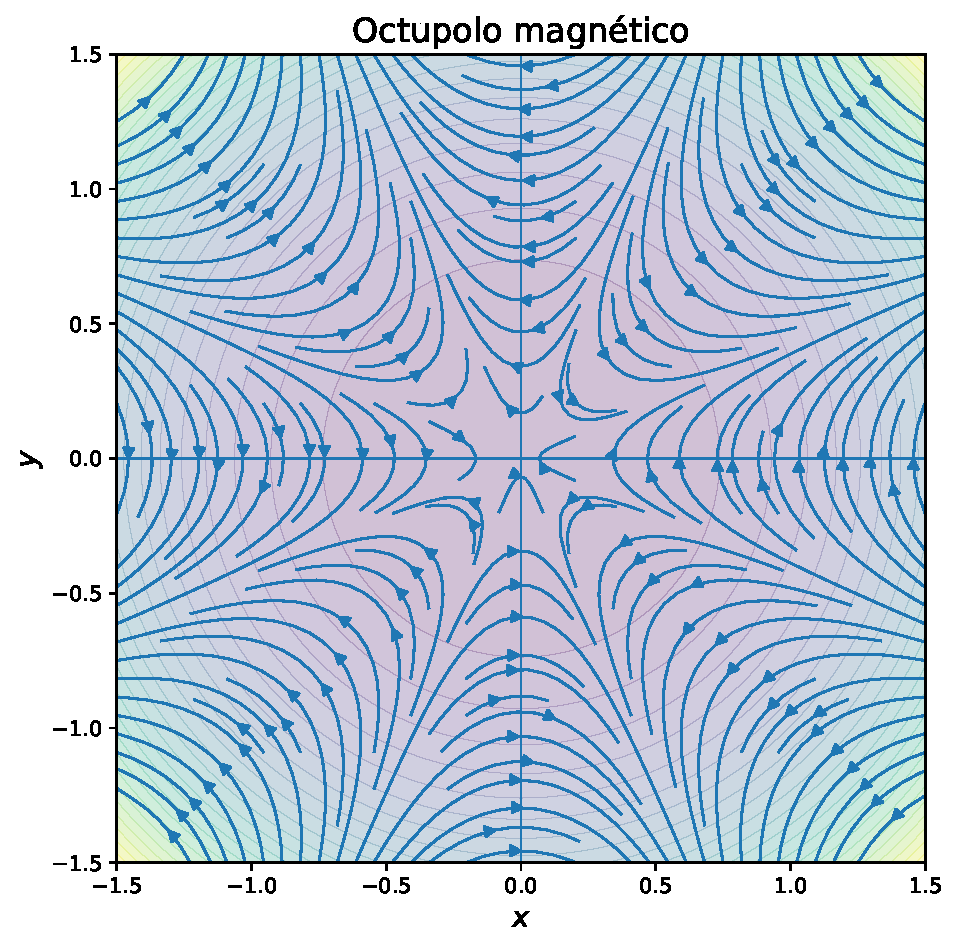
\includegraphics[width=0.85\linewidth]{octupolo_magnetico.pdf}
      \vspace{0.2cm}
      \textbf{Octupolo}
      \vspace{0.1cm}\small Correcciones no lineales
  \end{columns}
\end{frame}

\section{Dinámica del haz de partículas cargadas}
\begin{frame}{Trabajo nulo del campo magnético}
  La fuerza magnética sobre una carga $q$ con velocidad $\mathbf{v}$ es:
  \[
    \vec{F}_m = q(\vec{v} \times \vec{B})
  \]
  El trabajo diferencial $dW$ realizado por esta fuerza sobre un desplazamiento infinitesimal $d\mathbf{l} = \mathbf{v}\,dt$ es:
  \begin{align*}
    dW &= \vec{F}_m \cdot d\vec{l} \\
        &= q(\vec{v} \times \vec{B}) \cdot (\vec{v}\,dt) \\
        &= q\big[(\vec{v} \times \vec{B})\cdot \vec{v}\big]dt
  \end{align*}
  Por propiedades del producto mixto, el vector $(\vec{v} \times \vec{B})$ es ortogonal a $\mathbf{v}$, por lo que su producto escalar es cero:
  \[
    \boxed{dW = 0 \implies W = 0}
  \]
\end{frame}

\begin{frame}{Radio de curvatura}
  \begin{block}{Trayectoria del haz de partículas}
    Para $\vec{v}\perp\vec{B}$, la fuerza magnética actúa como fuerza centrípeta y curva la trayectoria.
  \end{block}

  \vspace{4mm}
  \begin{columns}[c]
    \column{0.5\textwidth}
      \centering
      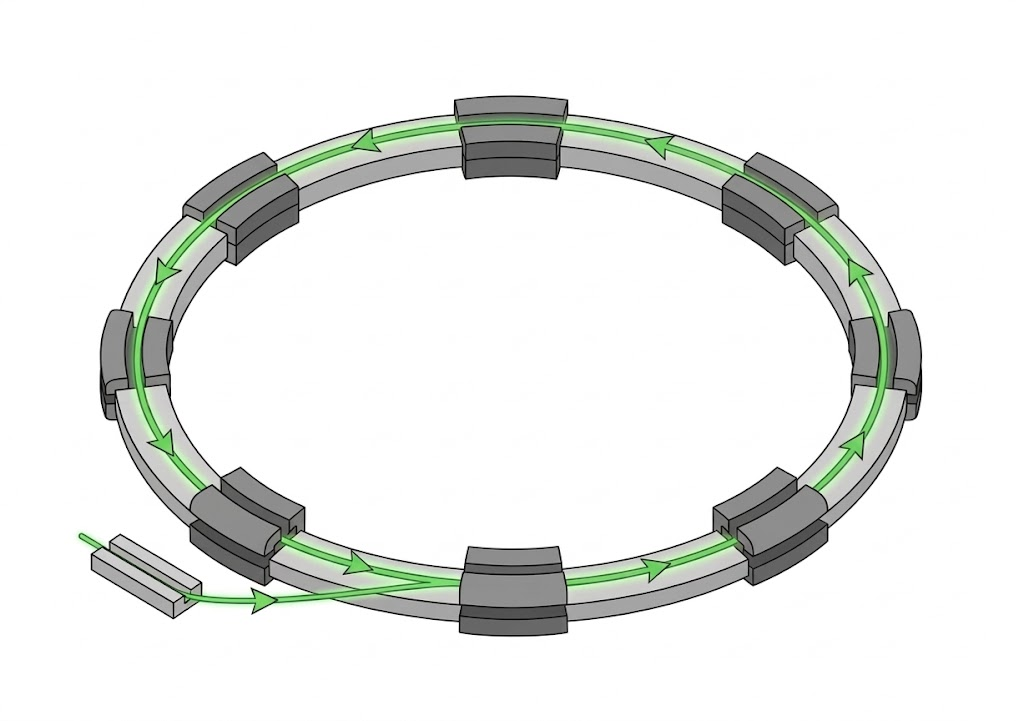
\includegraphics[width=0.9\textwidth]{trayectoria.png}
      \vspace{1mm}
      \tiny{\textit{$^7$Trayectoria del haz de partículas}}

    \column{0.25\textwidth}
      \[
        F_B = |q|vB
      \]
      \[
        F_c = \frac{mv^2}{R}
      \]
      \[
        |q|vB = \frac{mv^2}{R}
      \]

    \column{0.25\textwidth}
      \[
        |q|B = \frac{mv}{R}
      \]
      Sabemos que $p = mv$, de modo que:
      \begin{equation}
        R = \frac{p}{|q|B}
        \label{momento}
      \end{equation}
  \end{columns}
  \footnotetext[7]{Imagen generada con Gemini (Google), 2026.}
\end{frame}

\begin{frame}{El régimen relativista}
  \begin{block}{Velocidades extremas}
    En los aceleradores de partículas modernos, como los sincrotrones, las partículas alcanzan velocidades cercanas a la de la luz ($v \approx c$).
  \end{block}
  \[
    \gamma = \frac{1}{\sqrt{1-\beta^2}}, \quad \beta = \frac{v}{c}
  \]
  \begin{alertblock}{Radio de curvatura relativista}
    \begin{equation}
      R = \frac{p}{|q|B} = \frac{\gamma m v}{|q|B}
    \end{equation}
  \end{alertblock}
\end{frame}

\begin{frame}{Radiación emitida por una partícula cargada}
  \centering
  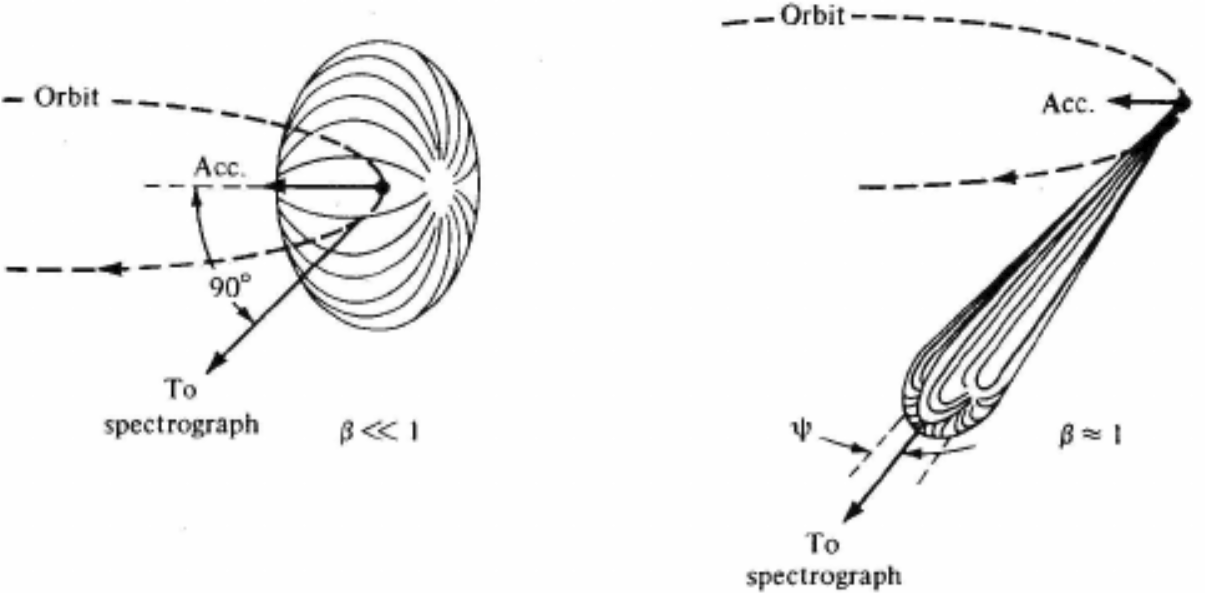
\includegraphics[width=0.7\textwidth]{image.png}
  \small $^8$Patrones cualitativos de radiación asociados a cargas que se desplazan en una órbita circular.
  \begin{block}{}
    Una partícula cargada eléctricamente emite radiación electromagnética cuando experimenta una aceleración.
  \end{block}
  \footnotetext[8]{Tomada de: Introduction to the main properties of Synchrotron Radiation - S. Mobilio and A. Balerna}
\end{frame}

\begin{frame}{Ángulo de apertura y colimación}
  \begin{block}{Semiángulo de apertura vertical ($\psi$)}
    \begin{equation}
      \psi \approx \frac{mc^2}{E} \approx \gamma^{-1}
      \label{eq:angulo_apertura}
    \end{equation}
  \end{block}
  \vspace{3mm}
  \textbf{Electrones y positrones}
  \[\gamma = 1957\text{ (GeV$^{-1}$)}\,E\text{ (GeV)}\]
  Para un anillo de almacenamiento operando a una energía de $E = 1\text{ GeV}$, el ángulo resulta ser:
  \[\psi \approx 0.5\text{ mrad}\]
  \footnotetext[5]{Ec. \ref{eq:angulo_apertura}: Introduction to the main properties of Synchrotron Radiation - S. Mobilio and A. Balerna}
\end{frame}

\begin{frame}{¿En dónde se encuentra la radiación sincrotrón en el espectro?}
  \centering
  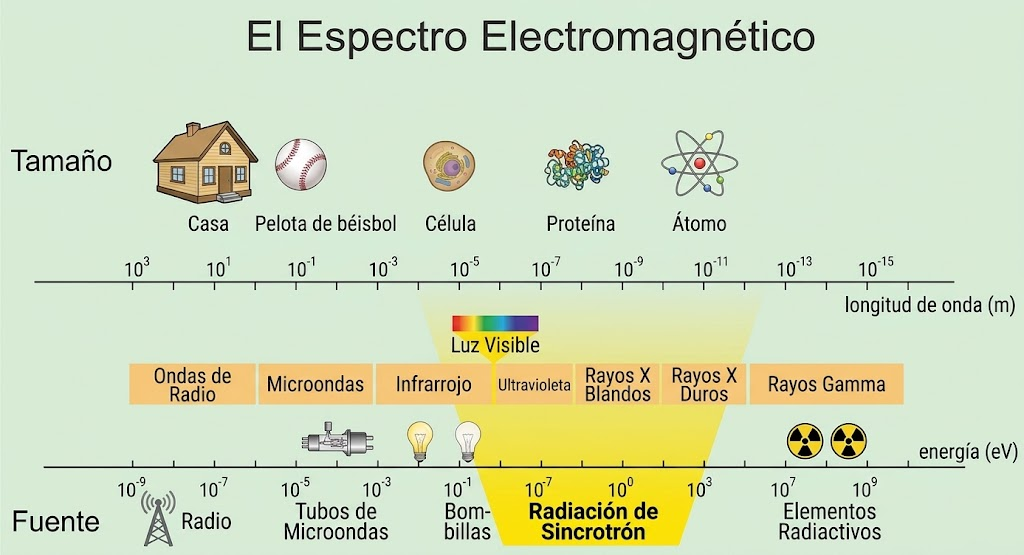
\includegraphics[width=0.7\textwidth]{espectro.png}
  \vspace{2mm}
  {\small \textit{$^9$Espectro electromagnético}}
  \footnotetext[9]{E. Kogan, \textit{Electrodynamics Course}. ResearchGate.}
\end{frame}

\section{Aplicaciones: XRD y SAXS}
\begin{frame}{XRD}
  \begin{block}{XRD (X-Ray Diffraction)}
    En español, \textcolor{red}{difracción de rayos X}, es una técnica analítica no destructiva para analizar propiedades físicas como la composición de fases, la estructura \textcolor{blue}{cristalina} y la orientación de muestras en polvo, sólidas y líquidas.
  \end{block}
  \begin{columns}
    \column{0.3\textwidth}
      \centering
      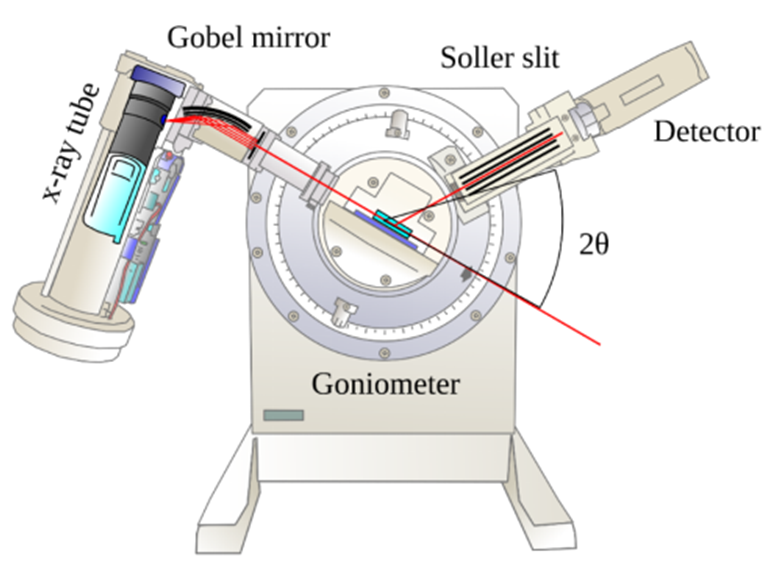
\includegraphics[width=\textwidth]{XRDdiagrama.png}
    \column{0.3\textwidth}
      \centering
      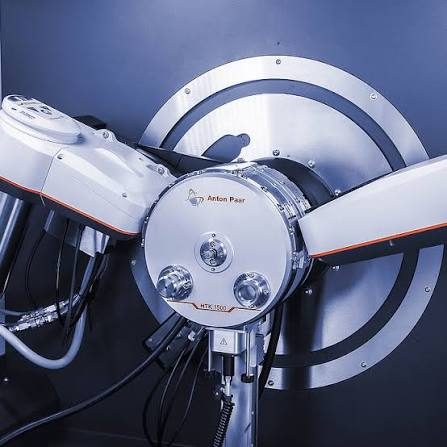
\includegraphics[width=\textwidth]{XRDe.jpg}
  \end{columns}
\end{frame}

\begin{frame}{¿Cómo funciona el método de difracción de rayos X?}
  \begin{block}{Los cristales como rendijas}
    Recordemos el experimento de la doble rendija de Thomas Young (1801). Al pasar una fuente de luz de ondas planas, se generan dos ondas radiales que terminan produciendo un patrón de interferencia.
  \end{block}
  \begin{columns}
    \column{0.3\textwidth}
      \centering
      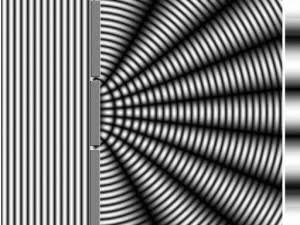
\includegraphics[width=\textwidth]{doblerem.jpg}
    \column{0.3\textwidth}
      \centering
      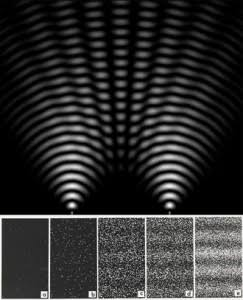
\includegraphics[width=\textwidth]{patrondeinterferencia.jpg}
  \end{columns}
\end{frame}

\begin{frame}{¿Cómo funciona el método de difracción de rayos X?}
  \begin{block}{¿Las cargas como rendijas o las rendijas como cargas?}
    Así como una onda plana se convierte en una onda radial al atravesar una rendija, ocurre algo análogo cuando la luz de sincrotrón incide sobre una carga. Su campo eléctrico oscilante obliga a la carga a oscilar.
  \end{block}
  \centering
  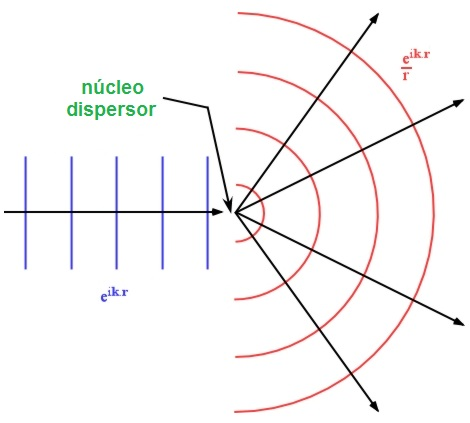
\includegraphics[width=0.3\textwidth]{onda incidente y onda esparcida.jpg}
\end{frame}

\begin{frame}{¿Qué es un cristal?}
  \begin{block}{Cristales}
    Los \textcolor{red}{cristales} son cuerpos sólidos constituidos por un conjunto de partículas (átomos, iones o moléculas) que están dispuestos según un \textcolor{blue}{orden regular y repetido}. Se forma así una red cristalina, una estructura tridimensional en la que se observa una sucesión ordenada de celdas elementales.
  \end{block}
  \begin{columns}
    \column{0.3\textwidth}
      \centering
      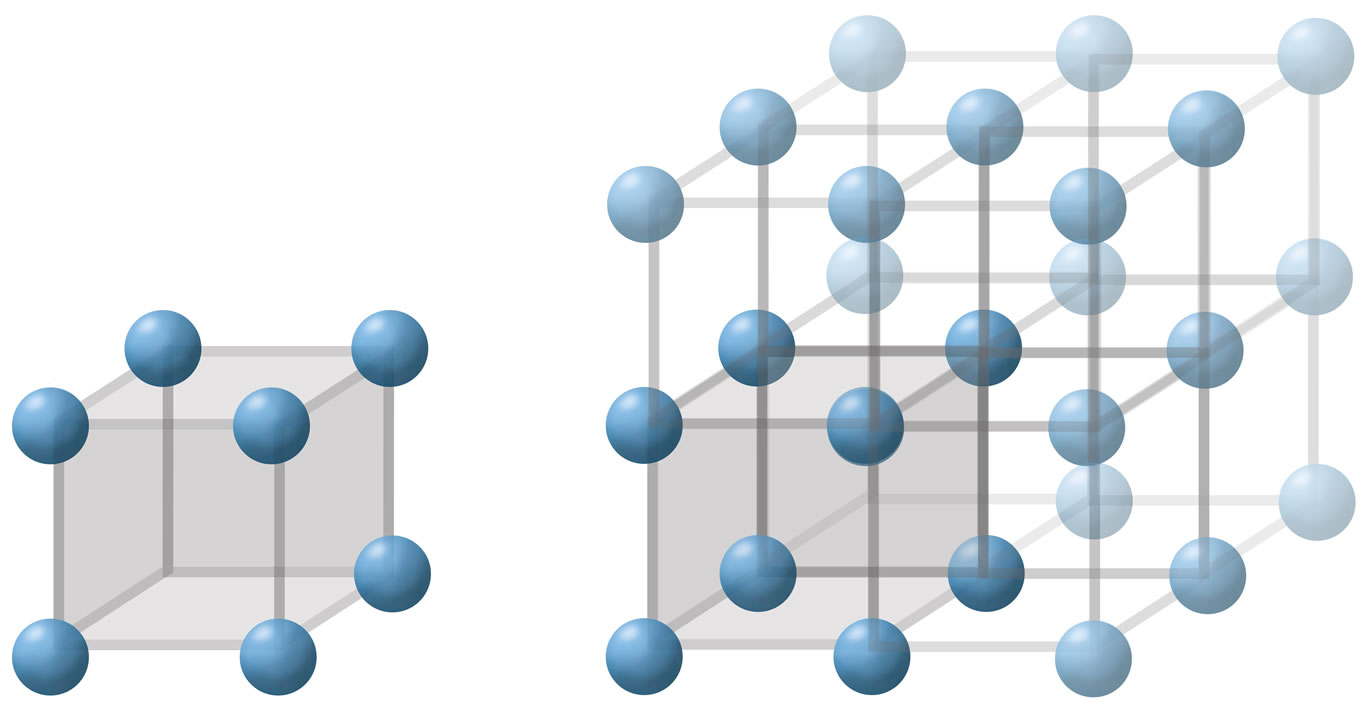
\includegraphics[width=\textwidth]{cristal-red-cristalina.jpg}
    \column{0.3\textwidth}
      \centering
      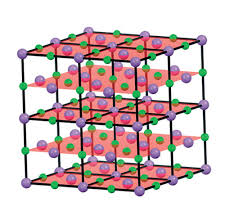
\includegraphics[width=\textwidth]{cristales.jpg}
  \end{columns}
\end{frame}

\begin{frame}[t]{Suma de carga (densidad electrónica)}
  \vspace{0.5cm}
  \begin{columns}[T]
    \begin{column}{0.48\textwidth}
      Factor de fase para un solo átomo
      \begin{equation*}
        e^{-iqr}
      \end{equation*}
      \begin{block}{Suma de amplitudes complejas}
        \small En un cristal con orden geométrico periódico, la onda total dispersada es la suma fasorial de todas las ondas individuales, considerando su desfase relativo.
      \end{block}
      \vspace{0.3cm}
      \begin{equation*}
        F(\Delta k)= \sum_j e^{-i\Delta k \cdot r_j}
      \end{equation*}
    \end{column}

    \begin{column}{0.48\textwidth}
      \begin{block}{Dependencia angular}
        \small El desfase entre ondas depende del vector de dispersión $\Delta k = k'-k$. Según el ángulo de observación, las ondas interfieren de forma constructiva o destructiva.
      \end{block}
      \vspace{0.2cm}
      \begin{center}
        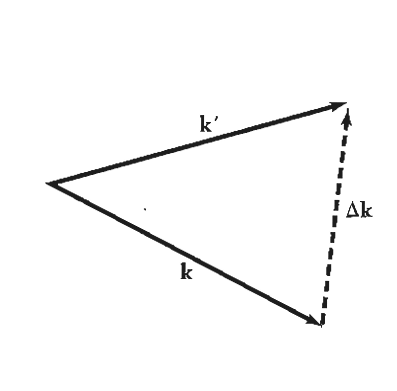
\includegraphics[width=0.5\textwidth]{k.png}
      \end{center}
    \end{column}
  \end{columns}
\end{frame}

\begin{frame}[t]{De la suma de cargas a la transformada de Fourier}
  \vspace{0.3cm}
  \begin{columns}[T]
    \begin{column}{0.48\textwidth}
      \begin{block}{De la suma discreta a la integral continua}
        \footnotesize Al describir los electrones como una densidad electrónica continua $n(\mathbf{r})$, la suma de todas las ondas esféricas re-radiadas se convierte en una integral de volumen:
        \vspace{0.2cm}
        \begin{equation*}
          F(\Delta\mathbf{k}) = \int n(\mathbf{r}) \, e^{-i\Delta\mathbf{k}\cdot\mathbf{r}} \, d^3r
        \end{equation*}
      \end{block}
    \end{column}

    \begin{column}{0.48\textwidth}
      \vspace{0.5cm}
      \begin{center}
        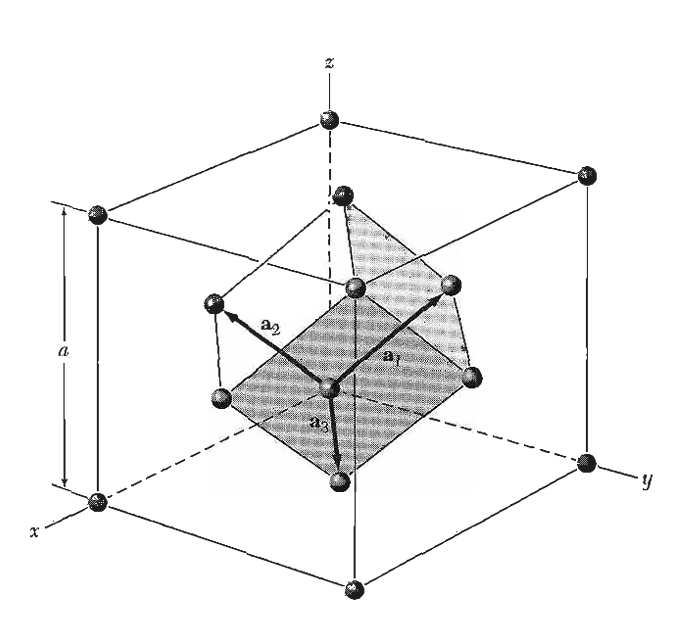
\includegraphics[width=0.8\textwidth]{reciproco.png}
      \end{center}
    \end{column}
  \end{columns}
\end{frame}

\begin{frame}[t]{Picos de Bragg}
  \begin{columns}[T]
    \begin{column}{0.5\textwidth}
      \begin{block}{Condición de difracción de von Laue}
        \begin{equation*}
          \Delta\mathbf{k} = \mathbf{G}
        \end{equation*}
      \end{block}
      \vspace{0.2cm}
      \small Siendo $\mathbf{G}$ el vector de la red recíproca.
      \vspace{0.4cm}
      La igualdad $\Delta\mathbf{k} = \mathbf{G}$ significa que el cristal solo puede absorber o ceder impulsos discretos $\mathbf{G}$, produciendo rayos dispersados únicamente en esas direcciones permitidas.
    \end{column}

    \begin{column}{0.48\textwidth}
      \begin{center}
        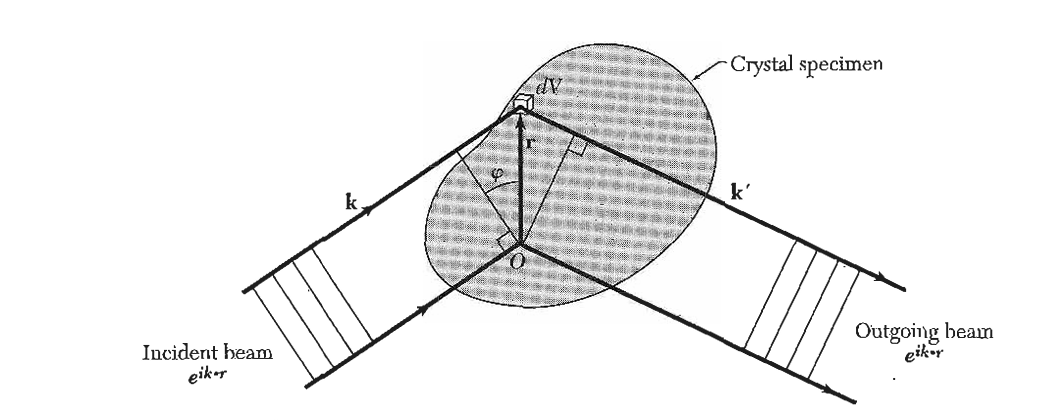
\includegraphics[width=0.8\textwidth]{bragg.png}
        \vspace{0.5cm}
        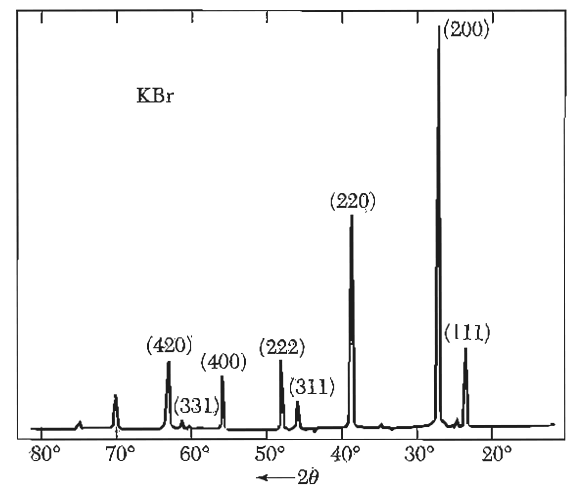
\includegraphics[width=0.6\textwidth]{Picosbragg.png}
      \end{center}
    \end{column}
  \end{columns}
\end{frame}

\begin{frame}[t]{SAXS: dispersión mesoestructural y transformada continua}
  \begin{columns}[T]
    \begin{column}{0.5\textwidth}
      \begin{block}{De átomos a nanoestructuras}
        \footnotesize Mientras que en XRD la "rendija" es la red atómica ($d \sim 1 - 10\,\text{\AA}$), en SAXS la rendija representa el contorno de nanoobjetos amorfos o discontinuidades mesoestructurales ($D \sim 1 - 100\,\text{nm}$).
      \end{block}

      \begin{block}{Transformada de Fourier continua}
        \footnotesize Al carecer de orden cristalino infinito, la respuesta se calcula mediante la transformada de Fourier continua del contraste de densidad electrónica $\Delta\rho(\mathbf{r})$:
        \begin{equation*}
          A(\mathbf{q}) = \int_V \Delta\rho(\mathbf{r}) \, e^{-i\mathbf{q}\cdot\mathbf{r}} \, d^3r
        \end{equation*}
      \end{block}
    \end{column}

    \begin{column}{0.45\textwidth}
      \vspace{1cm}
      \begin{center}
        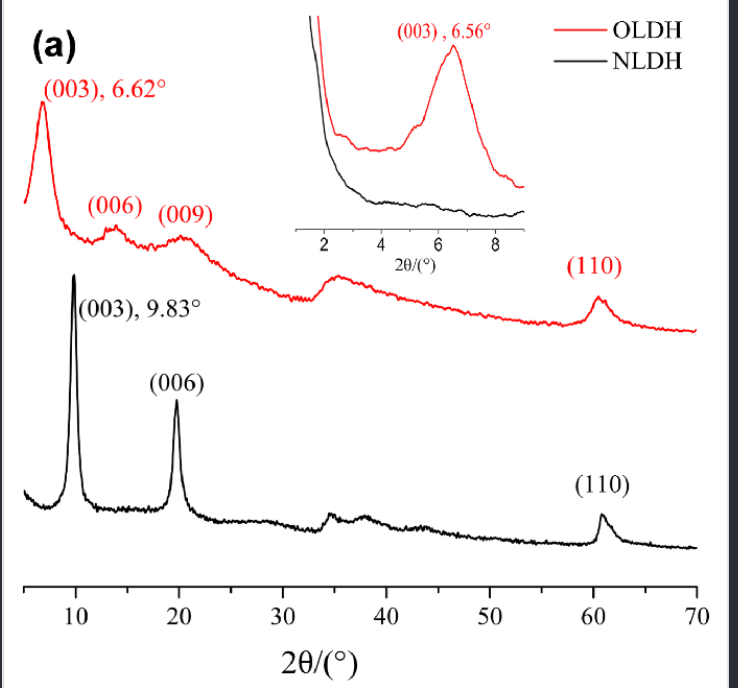
\includegraphics[width=0.8\textwidth]{xrdsaxs.png}
      \end{center}
    \end{column}
  \end{columns}
\end{frame}

\begin{frame}[t]{De la dispersión al espacio real}
  \begin{columns}[T]
    \begin{column}{0.52\textwidth}
      \begin{block}{Información física extraída}
        \footnotesize Determina distancias interatómicas promedio en líquidos y vidrios, la función de distribución $p(r)$ y el radio de giro $R_g$ de macromoléculas en solución.
      \end{block}
    \end{column}
    \begin{column}{0.44\textwidth}
      \vspace{1cm}
      \begin{center}
        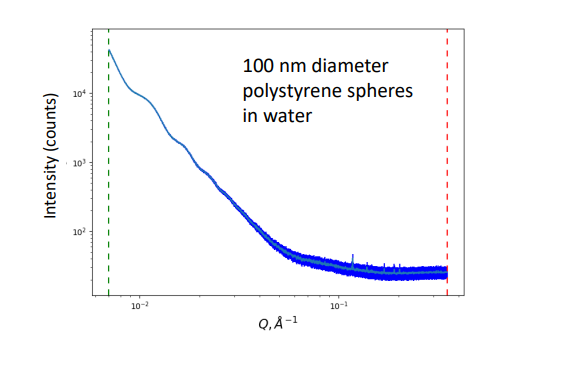
\includegraphics[width=\textwidth]{SAXS.png}
      \end{center}
    \end{column}
  \end{columns}
\end{frame}

\begin{frame}{Estudios realizados con luz de sincrotron}
  \begin{columns}[T]
    \column{0.48\textwidth}
      \centering
      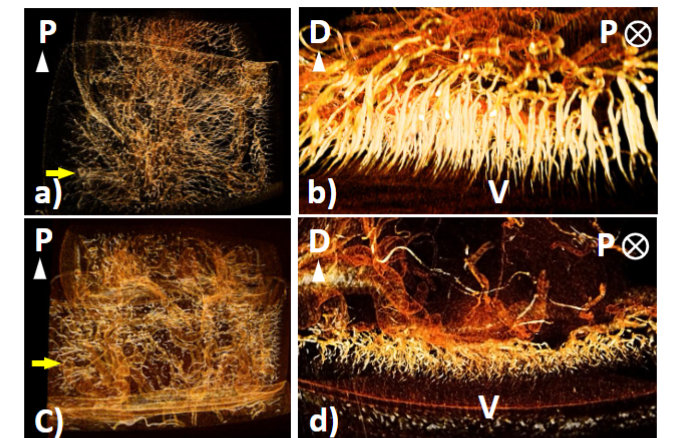
\includegraphics[width=\textwidth]{luciernagas.png}
    \column{0.38\textwidth}
      \vspace{1cm}
      \centering
      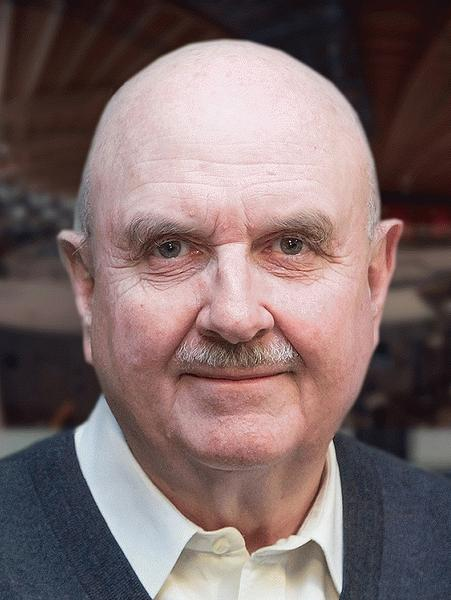
\includegraphics[width=0.6\textwidth]{gmaragaritondo.jpg}
  \end{columns}
\end{frame}

\begin{frame}{Estudios realizados con luz de sincrotron}
  \begin{columns}[T]
    \column{0.38\textwidth}
      \centering
      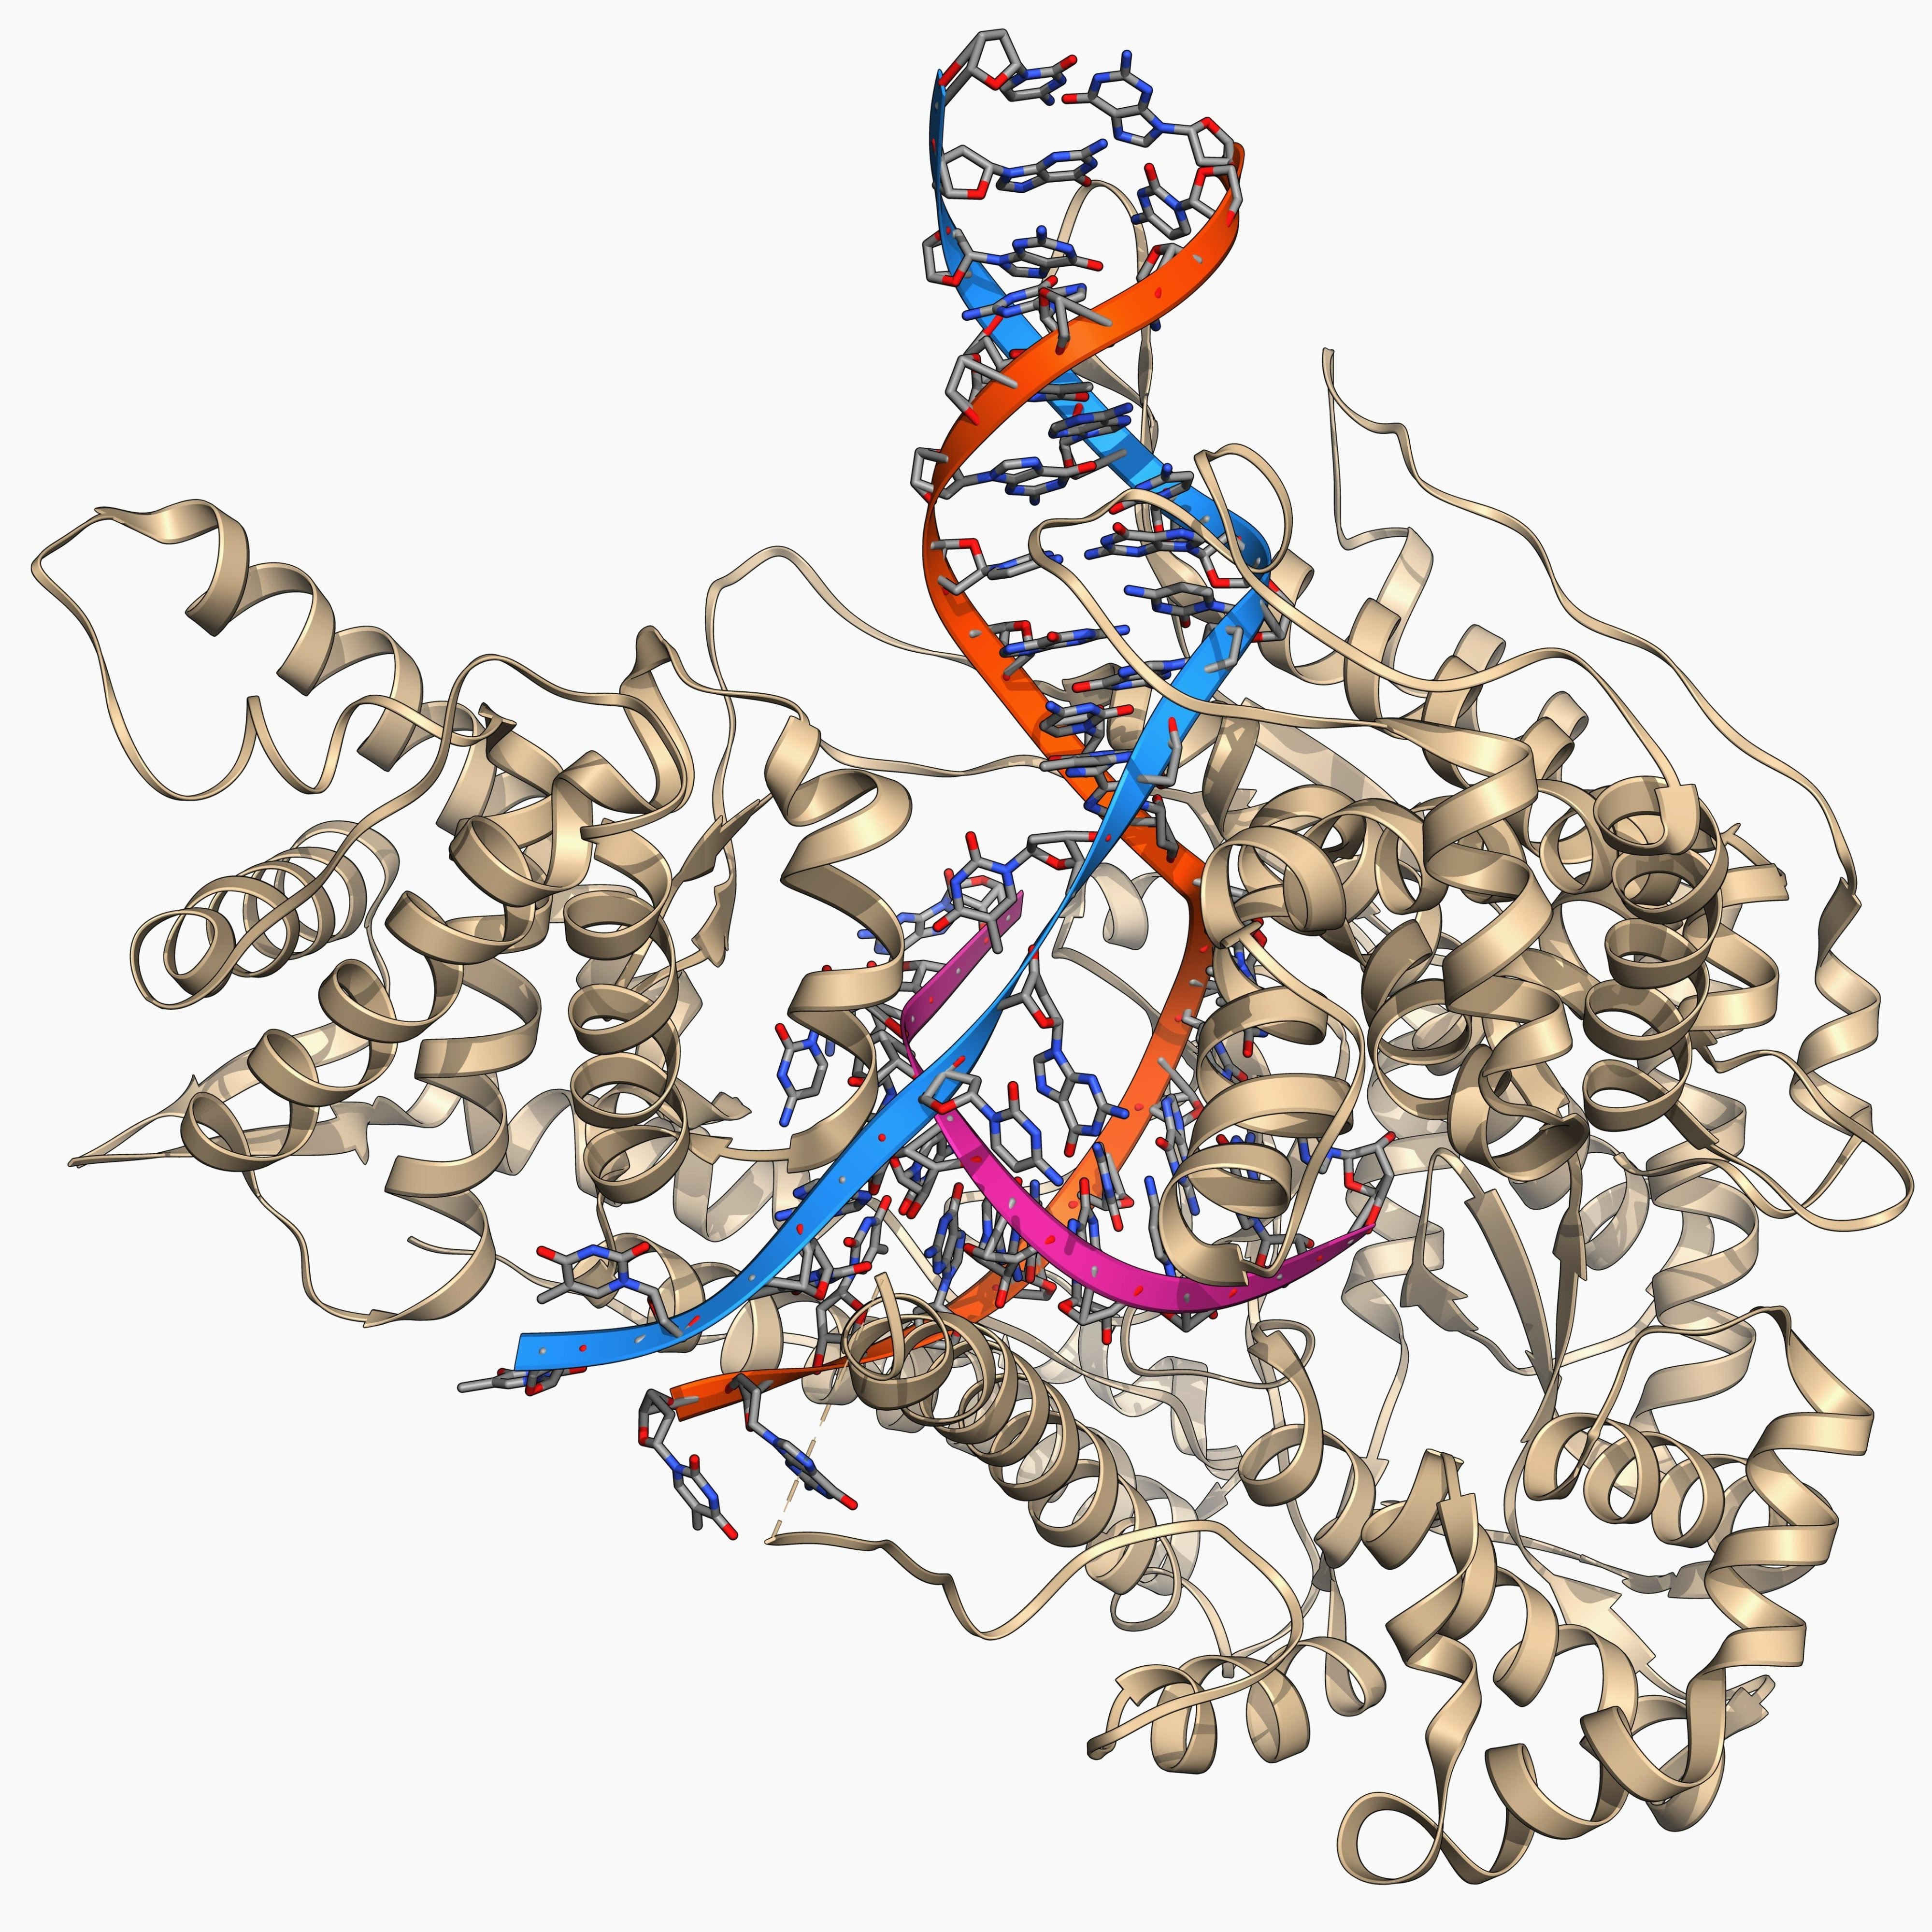
\includegraphics[width=\textwidth]{arn.jpg}
    \column{0.38\textwidth}
      \vspace{1cm}
      \centering
      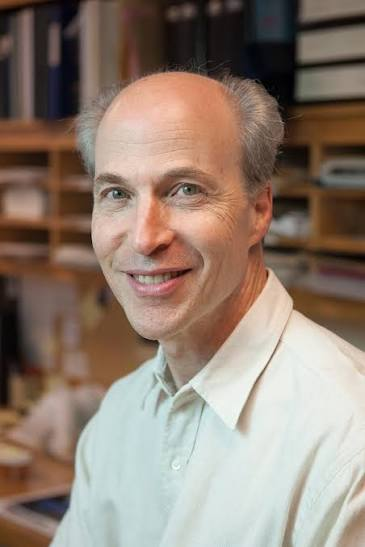
\includegraphics[width=0.6\textwidth]{nobel.jpg}
  \end{columns}
\end{frame}

\section{Conclusiones}
\begin{frame}{Conclusiones}
  \centering
  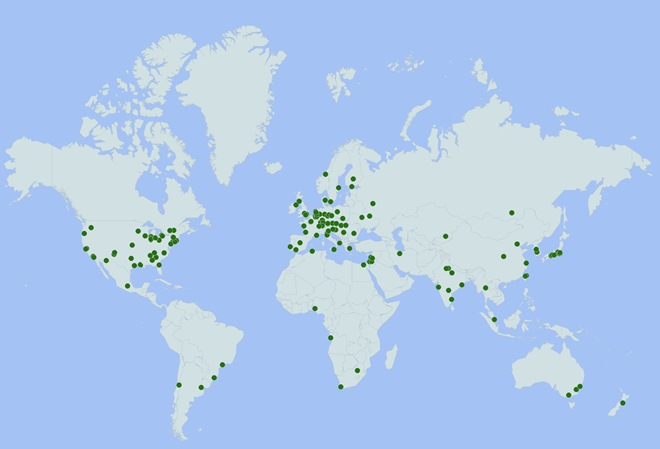
\includegraphics[width=0.7\textwidth]{mapasincrotrones.jpg}
\end{frame}



% ============================================================
% DIAPOSITIVA FINAL (AGRADECIMIENTOS Y PREGUNTAS)
% ============================================================

{
\setbeamertemplate{footline}{}
\setbeamertemplate{headline}{}

\begin{frame}[plain]
    \begin{tikzpicture}[remember picture,overlay]
        % FONDO AZUL INSTITUCIONAL
        \fill[UABlue] 
            (current page.south west) 
            rectangle 
            (current page.north east);

        % FRANJA NARANJA LATERAL (Para mantener la identidad visual)
        \fill[UAOrange]
            ([xshift=0.8cm]current page.north west)
            rectangle
            ([xshift=1.0cm]current page.south west);

        % TRIÁNGULO DECORATIVO DE FONDO (Sutil)
        \fill[White, opacity=0.03]
            (current page.south east) --
            ([yshift=7cm]current page.south east) --
            ([xshift=-10cm]current page.south east) -- cycle;

        % TEXTO PRINCIPAL: ¡GRACIAS!
        \node[
            anchor=west,
            text=White,
            font=\fontsize{25}{20}\selectfont\bfseries
        ]
        at ([xshift=2.0cm,yshift=1.5cm]current page.west)
        {
            ¡Gracias por su atención!
        };

        % TEXTO: ¿PREGUNTAS?
        \node[
            anchor=west,
            text=UAOrange,
            font=\fontsize{28}{34}\selectfont\bfseries
        ]
        at ([xshift=2.0cm,yshift=-0.2cm]current page.west)
        {
            ¿Preguntas?
        };

        % LÍNEA SEPARADORA
        \draw[White, thick, opacity=0.5]
            ([xshift=2.0cm,yshift=-1.2cm]current page.west) --
            ([xshift=13.0cm,yshift=-1.2cm]current page.west);

        % CORREOS ELECTRÓNICOS
        \node[
            anchor=west,
            text=White,
            align=left,
            font=\large
        ]
        at ([xshift=2.0cm,yshift=-2.2cm]current page.west)
        {
            \textbf{Contactos:}\\[0.2em]
            fmojeda@mail.uniatlantico.edu.co\\
            adeleond@mail.uniatlantico.edu.co
        };

        % LOGO DE LA UNIVERSIDAD (Opcional, en la esquina inferior derecha)
        \IfFileExists{UA.png}{
            \node[
                anchor=south east
            ]
            at ([xshift=-1.2cm,yshift=0.8cm]current page.south east)
            {
                
\includegraphics[height=2.2cm]{UA.png}
            };
        }{}
    \end{tikzpicture}
\end{frame}
}

\end{document}
